\subsubsection{19.03.2016}
\textit{\textbf{Time frame:}} 13:00-22:00 

The wheel base was assembled (figure \ref{Wheelbase4.1}). The chains were not held yet.

The gripper was connected to the 41,5 cm beams. The chains were not held yet.

It was created the second mount for the lifting mechanism (figure \ref{Winch4.5}) and the mechanism was connected to the robot (figure \ref{Robot1.1}, \ref{Robot1.2}).

It was created the mount for the mechanism for shifting the bucket. 

\begin{figure}[H]
	\begin{minipage}[h]{0.47\linewidth}
		\center{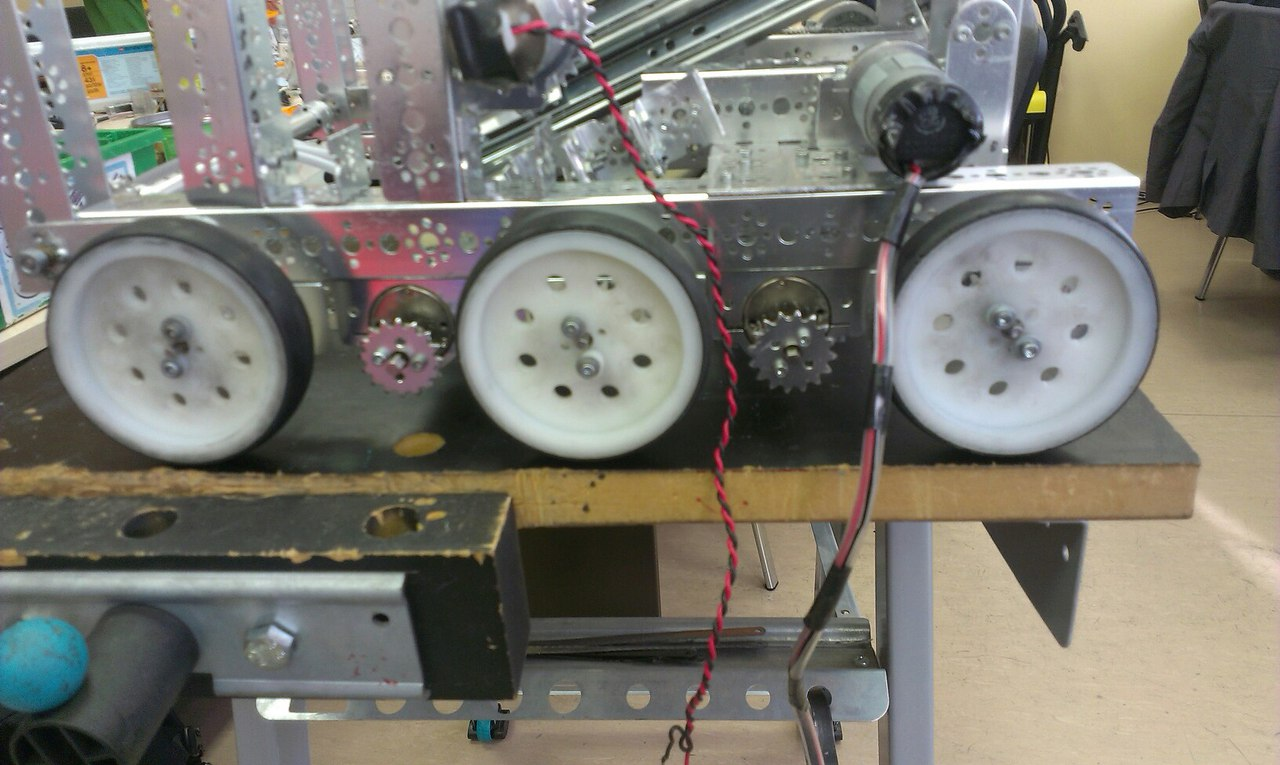
\includegraphics[scale=0.2]{3Engineering/5Team_meetings/days_of_meetings/2016.03.19/images/01}}
		\caption{Wheelbase without chains}
		\label{Wheelbase4.1}
	\end{minipage}
	\hfill
	\begin{minipage}[h]{0.47\linewidth}
		\center{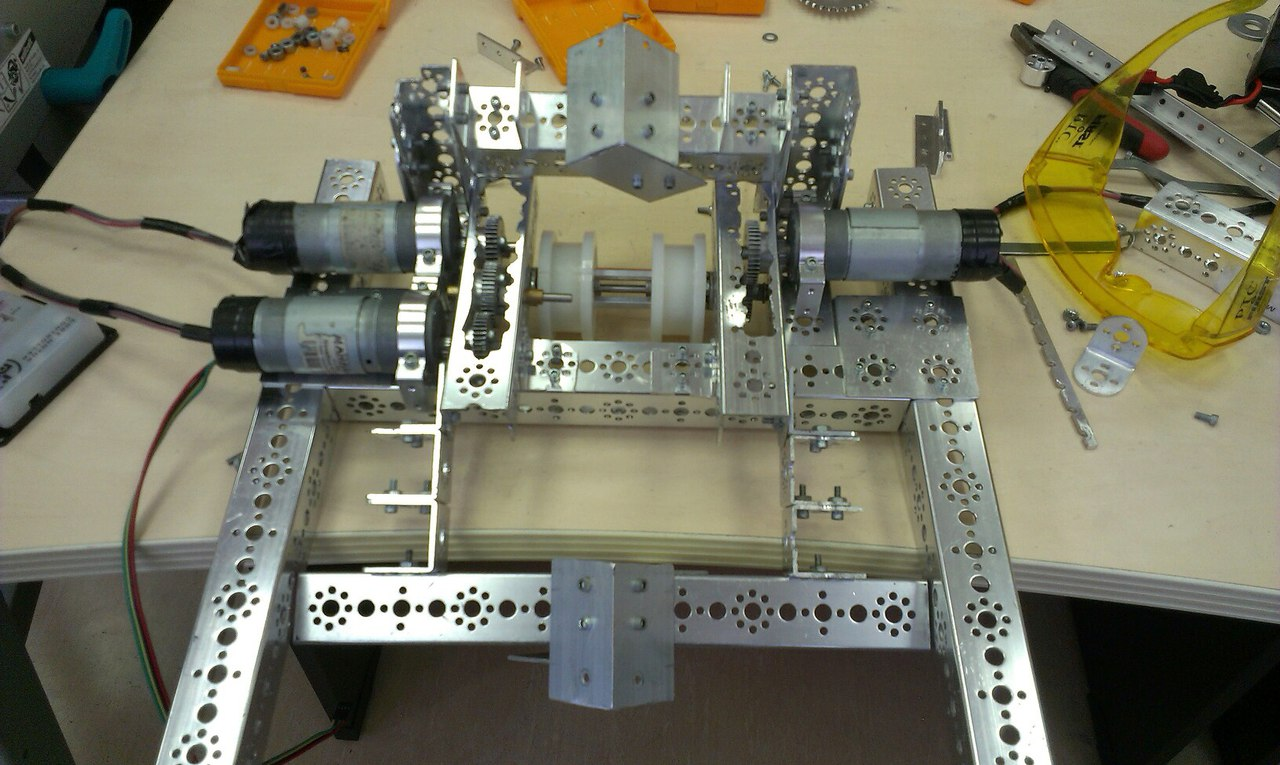
\includegraphics[scale=0.2]{3Engineering/5Team_meetings/days_of_meetings/2016.03.19/images/02}}
		\caption{The second mount for the lifting mechanism}
		\label{Winch4.5}
	\end{minipage}
	\vfill
	\begin{minipage}[h]{0.47\linewidth}
		\center{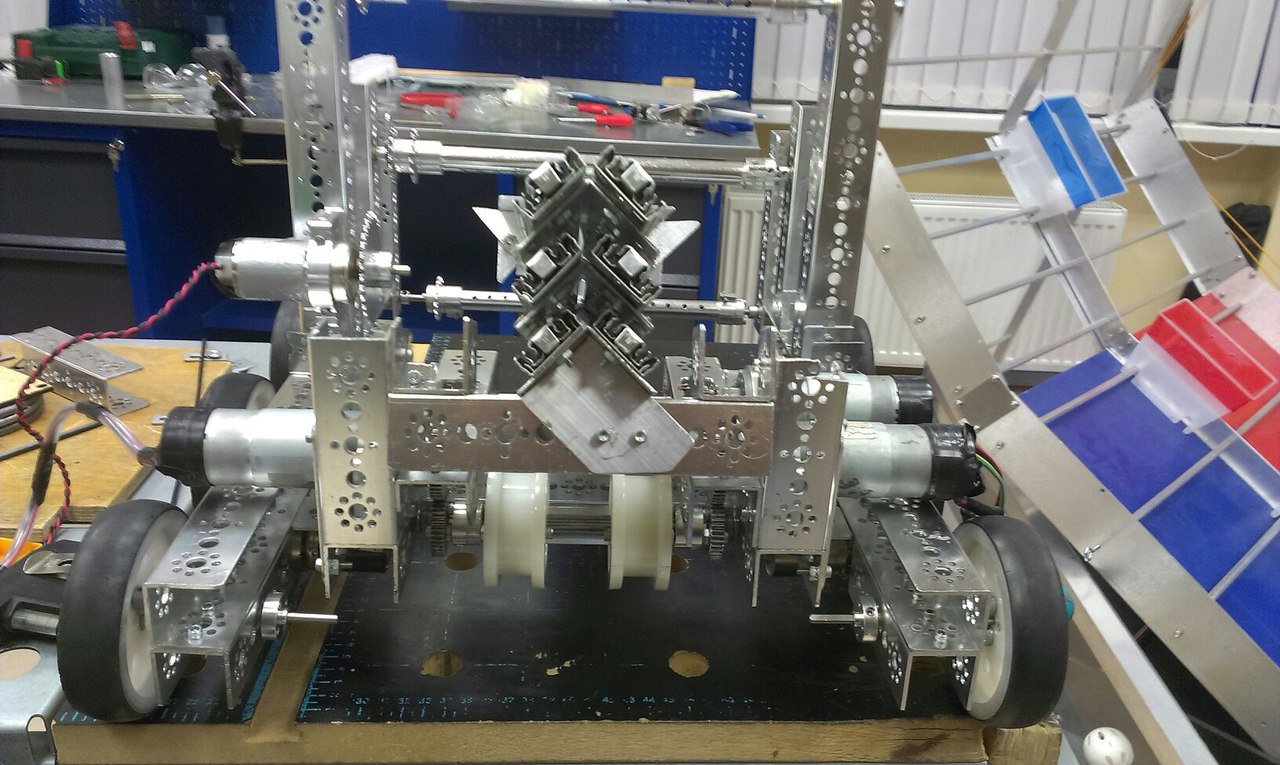
\includegraphics[scale=0.2]{3Engineering/5Team_meetings/days_of_meetings/2016.03.19/images/03}}
		\caption{New robot (back)}
		\label{Robot1.1}
	\end{minipage}
	\hfill
	\begin{minipage}[h]{0.47\linewidth}
		\center{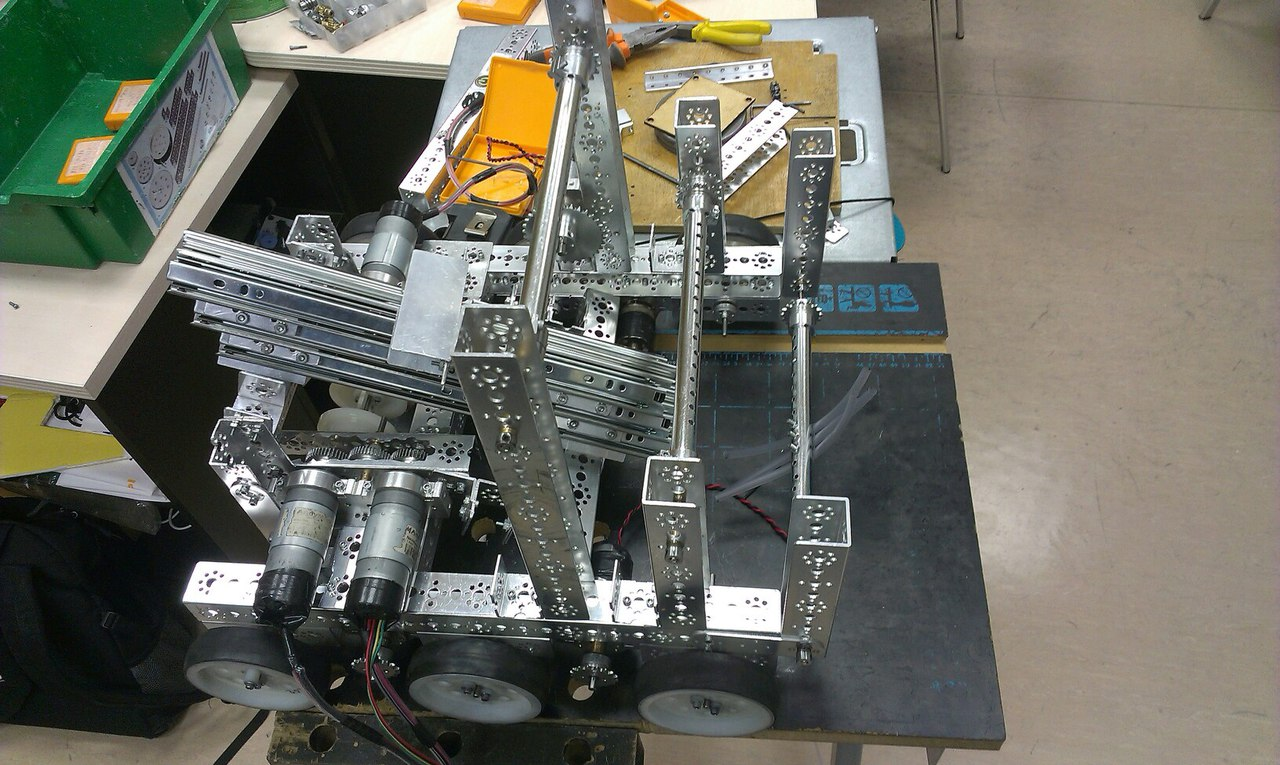
\includegraphics[scale=0.2]{3Engineering/5Team_meetings/days_of_meetings/2016.03.19/images/04}}
		\caption{New robot (side)}
		\label{Robot1.2}
	\end{minipage}
\end{figure}
